%
% File: chap03-03-01.tex
% Author: PINRU & LEONA
% Description:
% 3.3 Back-end Design and Implementations
%  3.3.1 API
%     Design
%     Implementation
%

\paragraph{Implementation}\mbox{}\\

During the implementation, we used Spring Boot 3.5.3 with MyBatis for the database operation, which follows the patterns of a layered architecture \cite{fowler2002}. We are writing the actual API requests based on the API specification instructions.

The majority of the APIs are built similarly. For annotations like @GetMapping, we can set the kind of request type it is, the path it uses, and the response it gives back. The function then safely collects user details and passes them to the service layer methods, for them to handle the request.

Example code is shown below about the patient appointment information:

\begin{figure}[h]
\centering
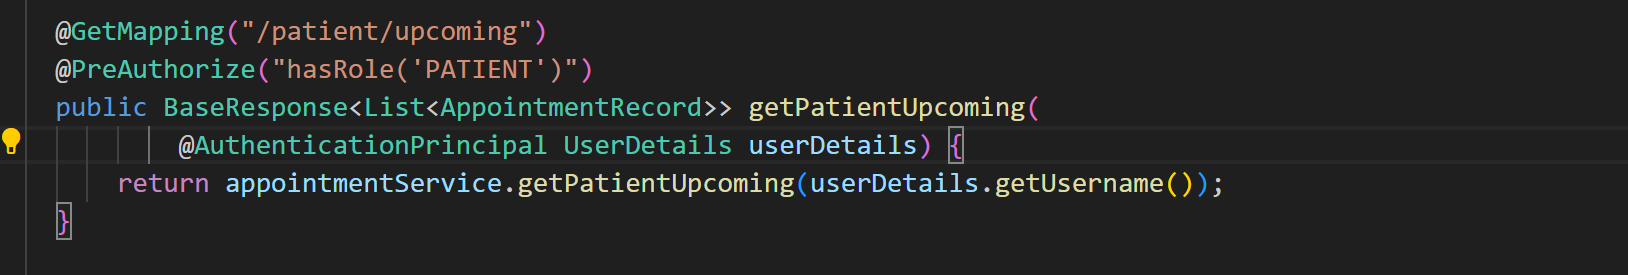
\includegraphics[width=0.8\textwidth]{chapters/chapter03/images03/3-3-1-figure(API-I).png}
\caption{Appointment Controller Implementation Code}
\label{fig:appointment-controller}
\end{figure}

Using @PreAuthorize, this will check the user's permissions and account levels \cite{springsecurity2024}. Using @AuthenticationPrincipal will then extract from Spring Security user information context; this doesn't need to authorise a token through a manual process \cite{johnson2023}.
The appointmentService.getPatientUpcoming() method includes dealing with business logic requests.

For the return type, we use \texttt{BaseResponse<T>}, replacing \texttt{ResponseEntity<ObjectNode>}, which offers the unified JSON structure. This type includes status code, message and data information, when dealing with different request errors, and the format makes it more consistent and clean.

Server methods contain business logic, and we use MyBatis to handle database operations \cite{springsecurity2024}. These functions create, update, delete, or query data through Mapper interfaces. MyBatis offer type-safe database operations and automatic SQL argument binding, compared to traditional JDBC, with fewer sample codes.

Some parts of server methods include more complicated logic, such as appointment scheduling, user personal information management, and health record handling. Those implementation methods not only enhance the optimisation, but also strengthen the system safety through Spring Security, integrate system safety, and provide a clear layer architecture to make the code more unified.
